\documentclass[runningheads]{llncs}
\usepackage{graphicx}
\usepackage{amsmath,amssymb} % define this before the line numbering.
\usepackage{ruler}
\usepackage{color}
\usepackage[width=122mm,left=12mm,paperwidth=146mm,height=193mm,top=12mm,paperheight=217mm]{geometry}

\usepackage{deform}

\begin{document}
% \renewcommand\thelinenumber{\color[rgb]{0.2,0.5,0.8}\normalfont\sffamily\scriptsize\arabic{linenumber}\color[rgb]{0,0,0}}
% \renewcommand\makeLineNumber {\hss\thelinenumber\ \hspace{6mm} \rlap{\hskip\textwidth\ \hspace{6.5mm}\thelinenumber}}
% \linenumbers
\pagestyle{headings}
\mainmatter
\def\ECCV12SubNumber{385}  % Insert your submission number here

\title{Learning Deformations with Parallel Transport} % Replace with your title

\titlerunning{ECCV-12 submission ID \ECCV12SubNumber}

\authorrunning{ECCV-12 submission ID \ECCV12SubNumber}

\author{Anonymous ECCV submission}
\institute{Paper ID \ECCV12SubNumber}


\maketitle


\begin{abstract}
    Many vision problems, such as object recognition and image
    synthesis, are greatly impacted by deformation of objects.
    In this paper, we develop a deformation model based on
    Lie algebraic analysis. This work aims to provide a
    generative model that explicitly decouples deformation from
    appearance, which is fundamentally different from
    the prior work that focuses on deformation-resilient
    features or metrics.
    %
    Specifically, the deformation group for each object can be
    characterized by a set of Lie algebraic basis. Such basis for
    different objects are related via parallel transport.
    Exploiting the parallel transport relations, we formulate an
    optimization problem, and derive an algorithm that jointly
    estimates the deformation basis for a class of objects, given a
    set of images resulted from the action of the deformations.
    %
    We test the proposed model empirically on both character
    recognition and face synthesis.
\end{abstract}

%%% Local Variables:
%%% TeX-master: "main_paper"
%%% End:



\section{Introduction}
\label{sec:introduction}

The changes in shapes of objects, often referred to as
\emph{deformations}, are widely observed in computer vision data.
In many problems, particularly object recognition based on appearance,
the performance can be greatly influenced by deformations. 
Whereas the past decades have seen tremendous efforts devoted to the
development of features and classifiers that are resilient to
variations of shapes and poses, the modeling of deformations has been
not been extensively explored. 
%
In this paper, we focus on modeling deformations, aiming to
develop a method that can decouple deformation from appearance of an
observed image. 

In past decades, a variety of approaches have been developed to
address the issue of deformations, for which we provide a brief review
in next section. Careful examination of previous shows that they are
limited in several aspects:
(1) While extensive research~\cite{ISO,LLE} has been performed on image
manifold modeling, this does not lead to effective modeling of deformations.
The problem here is that the differences between neighboring images
are due to the compound effects of deformations and other contributing
factors, and these approaches lack a mechanism to decouple the
effects.
(2) The methods for deformation-resilient
metrics~\cite{SC,IDM} aim to suppress the influence of deformation
on discriminative performance, which again does not offer an explicit
deformation model.
(3) Other work that explicitly takes deformations into
consideration~\cite{TD,HTrevor,ATV}
has a narrow focus on individual local tangent spaces, neglecting the
relations between them. As we will show, there are
significant dependencies between the different tangent spaces of the
deformation manifolds, which, if appropriately exploited,
contribute greatly to learning a model of deformation.

In this paper, we propose a new approach to deformation modeling,
where each observed image is considered to be generated by deforming
an object template. The observation of typical deformation patterns
exhibited in general images leads to the belief that most deformations
are well modeled by a low-dimensional Lie group, which can be characterized by
a basis of the associated Lie algebra. Intuitively, the Lie algebraic
basis captures the basic deformation patterns, and each deformation
in the group is some combination of them.
%
Generally, a different Lie algebra is associated with differing object
templates, which, however, are related to each other via the parallel
transport property. Specifically, the Lie algebra for one object
template is a transported version of the one for
others. The fact that parallel transport is covariant with geometric
transformation ensures the consistency of this relation.

Consequently, with the Lie algebraic characterization, the problem of learning
deformations reduce to the one of estimating the deformation basis
for different object templates. Here, we formulate an optimization problem
for estimating these bases from a given set of observed images. In
this formulation, two levels of relations are exploited:
(1) Observed images are closed to the deformation orbits, \ie~the
manifold is comprised of all deformed versions of the templates. 
(2) The basis associated with different templates are constrained by
the parallel transport relations.
The use of the first relation, which explicitly incorporates
deformation into the generative process of an image, clearly sets this
work apart from the large amount of prior work (\eg~those on image
manifold learning) that directly model the image space. Additionally,
the use of the parallel transport relation further distinguishes the
proposed approach from the methods which focus on local
neighborhoods only.

The remainder of this paper is organized as follows.
Section~\ref{sec:theory} reviews existing theoretrical results on deformations. The
emphasis is particularly placed on the Lie algebraic characterization
and parallel transport.
Section~\ref{sec:algorithm} formulates the optimization algorithm
for estimating the deformation model from observed images.
Emprirical results are presented in section~\ref{sec:experiments}, where we
compare the proposed method with related methods on character
recogition and synthesis, as well as face reconstruction.
Discussion of the method and results is provided in section~\ref{sec:conclusion}. 
%%% Local Variables:
%%% TeX-master: "main_paper"
%%% End:



\section{Related Work}
\label{sec:review}

We first briefly review previous work on deformations, which roughly
fall into two categories.
The first category of methods focuses on estimating global affine
transformation. Frey and Jojic~\cite{TMG1,TMG2,TMG3} proposes a
mixture model, where the space of affine transforms is discretized,
and an indicator is used to choose a specific transform in generating
each image.
Miller~\etal~\cite{Congeal} proposed a nonparametric probabilistic
model, which estimates the global affine transforms by gradually
aligning the images, using a gradient descent method referred to as ``congealing''.

The second category takes into account non-rigid deformations that can
lead to changes in shapes. Cootes~\etal~\cite{AAM,JP} proposed the
active appearance model for object alignment, where the deformation is
represented via the displacement of pre-specified control points.  In
addition, approaches by directly matching local descriptors are also
widely used.  Belongie et al.~\cite{SC} developed a direct matching
method using local shape context based on statistics of edges.  Keyser
et al.~\cite{IDM} developed an Image Distortion Model
(IDM)~\cite{IDM}, which pursues a dense match of local patches between
two images as a representation of the deformation.  Though simple,
this method leads to substantial improvement on character recognition,
providing significant evidence as to the important role of local
deformations in object recognition.  The pioneering work by
Tenenbaum~etal~\cite{ISO} and Roweis and Saul~\cite{LLE} initiated a
large amount of work that directly models the image manifold via
embeddings it into local low-dimensional spaces.

While deformation information is made use of in building object
metrics in the work mentioned above, these methods do not establish
an explicit model of deformations. Recently, new models have been
proposed to address this issue.
Simard et al.~\cite{TD} considered the manifold of deformations,
approximating it via local tangent spaces. In this work, the
basis of these tangent spaces are hand-crafted, with some apparent
deformation patterns taken into account (\eg~rotation and changes of
thickness). However, some subtle variations of shapes are difficult to
capture via manually devised patterns.
Another drawback of this method lies in the introduction of tangent
spaces for all training samples, incurring unnecessary
computational costs in both training and testing phases when the
samples are dense.
%
Hastie and Simard~\cite{HTrevor,ATV} improve upon this method by
grouping nearby samples into clusters and deriving the tangent basis
via learning. However, learning is performed independently for each
tangent space, utilizing only the samples within a local neighborhood.
This makes it potentially difficult to obtain reliable estimations. 
%%% Local Variables:
%%% TeX-master: "main_paper"
%%% End:










\section{The Theory of Deformation}
\label{sec:theory}

Generally, the shape and size of an non-rigid object can change over
time. Such a change is often referred to as a \emph{deformation},
which is ubiquitous in vision problems.
In this paper, we focus on the two-dimensional image space, where a
deformation can be formalized as a
\emph{diffeomorphic transform} on the image plane.

\begin{figure}[t]
    \centering
    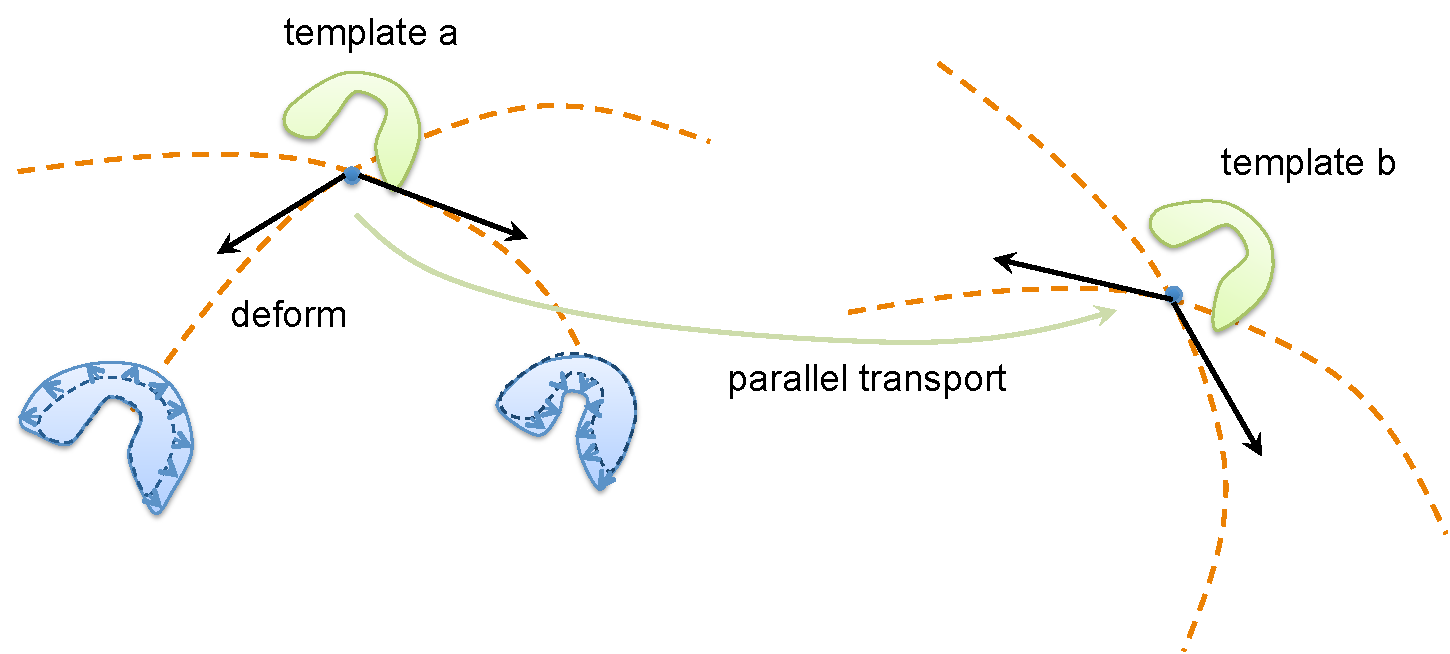
\includegraphics[width=0.8\textwidth]{deform_show.pdf}
    \caption{This figure illustrates the Lie algebraic
      characterization of deformation groups. Here, starting from an
      object template, a deformed image can be generated following a
      velocity field, which can be expressed as a linear combination
      of some basic patterns (captured by the Lie algebraic basis).
      The basis associated with different object templates are related
      by parallel transport. 
    }
    \label{fig:deform_show}
\end{figure}


\subsection{Lie Group and Lie Algebra}

Deformations typically observed in vision problems are a subset of all
diffeomorphic transforms, which we assume constitute a Lie group of
dimension $K$. A Lie group $G$ is a finite-dimensional manifold with
an algebraic group structure, meaning that it has the following
properties:
\begin{enumerate}
    \item The identity transform is in $G$.
    \item If $T_1$ and $T_2$ are both in $G$, then the
    composition $T_1 \circ T_2$ is also in $G$.
    \item For each transform $T \in G$, the inverse transform $T^{-1}$
    also exists in $G$.
\end{enumerate}
The Lie group $G$ is associated with a Lie algebra $\ga$, a vector space of
dimension $K$. Each vector $V \in \ga$ is a velocity field and
corresponds uniquely to a transform $T \in G$ via the exponentiation
mapping as below
\begin{equation}
    T = \exp(V).
\end{equation}
Here, $V$ is called the \emph{Lie algebraic representation} of $T$. 

The relations between a Lie group $G$ and its
associated Lie algebra $\ga$ can be described through the construction
of a continuous transformation process.
Let $V \in \ga$, then for every $t > 0$, $T_t = \exp(t V)$ is a
transform. Hence, the function below defines a trajectory on the image
plane.
\begin{equation} \label{eq:xt0}
    \vx(t) = T_t \vx_0 = \exp(t V) \vx_0.
\end{equation}
Intuitively, this trajectory can be generated through a continuous
transformation process described as follows.
Consider a particle starting from $\vx_0$. If the particle travels
across the image plane, passing through each location $\vx(t)$ with
velocity $V(\vx(t))$, the resultant trajectory is then given by
\begin{equation}
    \vx(t) = \vx_0 + \int_{\tau=0}^t V(\vx(\tau)) d\tau.   
\end{equation}
This provides a detailed characterization of the trajectory defined in
Eq.\eqref{eq:xt0}, namely $\exp(tV) \vx_0$.
Therefore, the transform $\exp(tV)$ can be understood as an operation
that sends each point to move for time $t$, following the velocity
field $V$.
Equivalently, the trajectory is characterized by the differential
equation below
\begin{equation}
    \frac{d \vx(t)}{dt} = V(\vx(t)).
\end{equation}
%
Given a basis of $\ga$, denoted by $\bset = (B_1, \ldots, B_K)$, each
Lie algebraic vector $V \in \ga$ can be expressed as a linear
combination as $V = \sum_{k=1}^K \alpha^k B_k$. As illustrated by
Figure~\ref{fig:deform_show}, each
base vector of $\ga$ reflects a basic deformation pattern, and all
deformations in $G$ are combinations of such base patterns. The Lie
algebraic characterization provides a representation, where such
combinations can be done via linear operations, great simplifying the
modeling and estimation.


\subsection{The Action on Images}

A deformation $T \in G$ can act on an image by moving the locations of
pixels. Let $I$ be an image. Applying $T$ to $I$ results in an
deformed image $T \circ I$, given by
\begin{equation}
    (T \circ I)(\vx) = I(T^{-1} \vx).
\end{equation}
This means that the pixel value of $T \circ I$ at $\vx$ equals that of
$I$ at $T^{-1} \vx$.
Let $V \in \ga$. Applying a continuous transform process $\exp(tV)$ to
the image $I$ yields a continuous sequence of images, as
\begin{equation}
    I_t(\vx) = (\exp(tV) \circ I)(\vx)
    = I(\exp(-tV) \vx).
\end{equation}
Taking the derivative \wrt~$t$, we get
\begin{equation} \label{eq:liealg_action}
    \left. \frac{d I_t(\vx)}{dt} \right|_{t=0}
    = - V(\vx)^T \nabla I(\vx)
    \triangleq (V \circ I) (\vx).
\end{equation}
Here, $V \circ I$ denotes the \emph{action of $V$ on $I$}, which
produces a scalar map, whose value at $\vx$ equals the negated inner
product between the velocity $V(\vx)$ and the image gradient
$\nabla I(\vx)$. Clearly, the action of $V$ is a linear operation on
$I$.

Given a basis $\bset$, we can write $V$ in form of a linear
combination as $V = \sum_{k=1}^K \alpha^k B_k$. Consequently, we can
rewrite Eq.\eqref{eq:liealg_action} into
\begin{equation} \label{eq:liealg_actiond}
    \left. \frac{d I_t(\vx)}{dt} \right|_{t=0}
    = \sum_{k=1}^K \alpha^k (B_k \circ I)(\vx).
\end{equation}
This equation establishes the linear isomorphism between the Lie
algebraic representation and the image changes due to deformation.
In other words, the infinitesimal changes due to a deformation, 
whose Lie algebraic representation is a linear combination of some
base deformations, can be expressed as the same linear combination of
the ``base changes'', \ie~those generated by the base deformations.
As we would see in next section, we rely on such decomposition for
model estimation from given images.



\subsection{Parallel Transport}

In general, a deformation group is associated with a specific object,
which can not be directly applied to a different object (\eg~a
transformed version of the object).
However, one can adapt a deformation group via the
\emph{parallel transport} of the associated Lie algebra, enabling its
application to different objects.

Consider an object being deformed, which are observed from two
different views. The point at $\vx$ from the first view is transformed
to $\vx' = T \vx$ from the second view. 
Suppose this point has velocity $\vv$ at $t = 0$ from the
first view, then \emph{what is the velocity of the corresponding
  point, \ie~$T \vx$, from the second view?}
The derivation below shows the answer:
\begin{equation}
    \vv' :=
    \lim_{\delta t \ato 0} \frac{T(\vx + \vv \delta t) -
      T(\vx)}{\delta t}
    = \mJ_T(\vx) \vv.
\end{equation}
Here, $\mJ_T(\vx)$ is the Jacobian matrix of $T$ at $\vx$. Here $\vv'$
is called the \emph{parallel transport} of $\vv$ \wrt~the transform
$T$. The parallel transport can be applied to an entire velocity field
$V$, resulting in a new velocity field $T \tsp V$, given by
\begin{equation}
    (T \tsp V)(T \vx) =
    \mJ_T(\vx) V(\vx).
\end{equation}
The parallel transports are \emph{covariant} with the inducing
transforms, meaning that they satisfy two properties below:
(1) the parallel transport induced by an identity transform in itself
is an identity, and
(2) the parallel transport induced by a composition of two transforms
equals the composition of the transports respectively induced, as
$(T_2 T_1) \tsp V = T_2 \tsp (T_1 \tsp V)$.




%%% Local Variables:
%%% TeX-master: "main_paper"
%%% End:


\section{Model Estimation Algorithm}
\label{sec:algorithm}

In this section, we formulate an optimization problem to estimate the
deformation groups for a specific class of objects, given a set of
images, and thereon derive an algorithm that jointly solves the basis
of the deformation groups and the Lie algebraic coefficients for the
training samples. 

\subsection{Two-Level Formulation}

\begin{figure}[t]
    \centering
    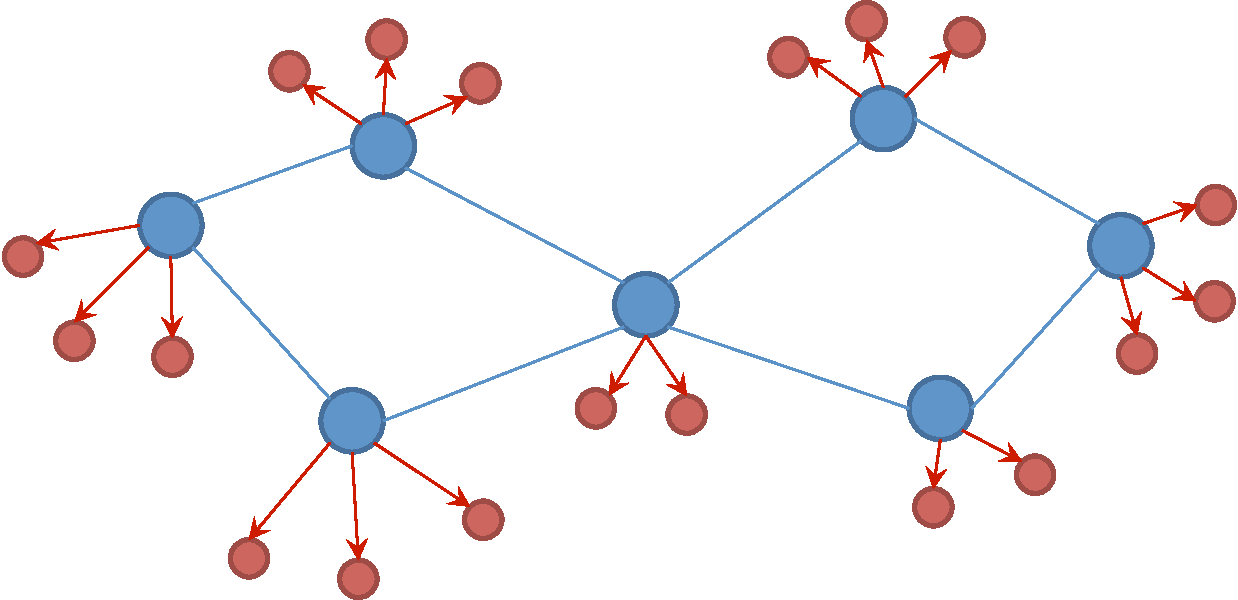
\includegraphics[width=0.8\textwidth]{pt_show.pdf}
    \caption{This figure shows the two-level formulation of the
      proposed optimization formulation. At the first level, each
      center image (depicted by blue circles) are connected to all its
    neighbors (red circles) within the same cluster, and at the second level,
    different centers are connected via parallel transport
    contraints. }
    \label{fig:pt_show}
\end{figure}


Given a set of $n$ images, we first group them into
$m$ clusters, using K-medoid, where each cluster has a \emph{center
  image}. The number of clusters $m$ is choosen via cross validation,
such that all samples within a cluster are close enough to the
corresponding center.
Suppose the $i$-th cluster contains $n_i$ samples. For this cluster, 
we use $I_{i,0}$ to denote the center image of this, and $I_{i,j}$
(with $j = 1, \ldots, n_i$) to the $j$-th non-center image. 
%
Here, we consider each center image as the representation of the canonical
shape of an object, and other images in the same cluster as generated
by deforming the center image.

As discussed in previous section, a deformation group can be
characterized by a Lie algebra. Therefore, the problem of learning the
deformation groups thus reduces to the one of estimating the Lie
algebraic basis for each cluster. Here, we denote the basis for the
$i$-th cluster by $\bset_i = (B_{i,1}, \ldots, B_{i,K})$.
To estimate these basis, we formulate an optimization problem, of
which the objective function comprises two levels of terms, as shown
in Figure~\ref{fig:pt_show}.


\subsubsection{Within-cluster Level.}
%
Applying the deformation group characterized by the Lie
algebraic basis $\bset_i$ to the image $I_{i,0}$ yields a
$K$-dimensional manifold comprised of all the deformed images,
denoted by $G(\bset_i) \circ I_{i,0}$, as
\begin{equation}
    G(\bset_i) \circ I_{i,0} \triangleq
    \{ \exp(V) \circ I_{i,0}: V \in \ga(\bset_i) \}.
\end{equation}
Here, $\ga(\bset_i)$ denotes the Lie algebraic space spanned by
$\bset_i$.
With the assumption that $I_{i,j}$ is generated by deforming
$I_{i,0}$, we expect that the $I_{i,j}$ is close to
$G(\bset_i) \circ I_{i,0}$. Particularly, the distance from $I_{i,j}$
to $G(\bset_i) \circ I_{i,0}$ is given by
\begin{equation}
    \dist(I_{i,j}, G(\bset_i) \circ I_{i,0})
    = \min_{\valpha} \left\| I_{i,j} -
      \exp \left(\sum_{k=1}^K \alpha^k B_{i,k} \right) \circ I_{i,0}
    \right\|.    
\end{equation}
When the deformed image $I_{i,j}$ is close to the center $I_{i,0}$,
the coefficients are small. Consequently, by
Eq.\eqref{eq:liealg_actiond}, we can approximately write
\begin{equation}
    \exp \left( \sum_{k=1}^K \alpha^k B_{i,k} \right) \circ I_{i,0}
    \simeq
    I_{i,0} + \sum_{k=1}^K \alpha^k (B_{i,k} \circ I_{i,0}).
\end{equation}
As a result, we have
\begin{align} \label{eq:approx_dist2}
    \dist(I_{i,j}, G(\bset_i) \circ I_{i,0})^2
    &\simeq
    \min_{\valpha} \left \|
      (I_{i,j} - I_{i,0}) -
      \sum_{k=1}^K \alpha^k (B_{i,k} \circ I_{i,0})
    \right \|^2 \notag \\
    &=
    \min_{\valpha} \sum_{\vx \in \dset} \left(
      (I_{i,j}(\vx) - I_{i,0}(\vx)) +
      \sum_{k=1}^K \alpha^k B_{i,k}(\vx)^T \nabla I_{i,0}(\vx)
    \right)^2.
\end{align}
Here, $\dset$ is the set of all observable pixel locations.
For convenience, we define
\begin{equation}
    Q_{ij}(\bset_i, \valpha_{i,j}) =
    \left \| (I_{i,j} - I_{i,0}) -
      \sum_{k=1}^K \alpha_{i,j}^k (B_{i,k}
      \circ I_{i,0})
    \right \|^2.
\end{equation}
Note that $Q_{ij}$ is a quadratic \wrt~$\valpha_{i,j}$. Hence, the
optimal coefficients that yield the minimum (approximate) distance can
be readily solved, given $\bset_i$.


\subsubsection{Inter-Cluster Level.}
%
The basis associated with different groups are related to each other
via parallel transport. Specifically, we establish a higher-level
network between cluster centers, where each center image is connected
to several \emph{neighboring centers}, \ie~other centers that are not
too far from it, such that the optical flow between them can be
reliably estimated.

For each pair of neighboring centers $I_{i,0}$ and $I_{i',0}$, we
estimate the dense correspondence between them $T_{ii'}$ and
$T_{i'i}$, using an optical flow algorithm~\cite{OF}.
Ideally, we would expect the basis $\bset_{i}$ to be the transported
version of $\bset_{i'}$ \wrt~the transform $T_{i'i} = T_{ii'}^{-1}$,
\ie~$B_{i,k} = T_{ii'}^{-1} \tsp B_{i',k}$, and vice versa. As some errors
may be incurred in optical flow estimation, we use the quadratic term as
follows to penalize the deviation from this relation:
\begin{equation}
    H_{ii'}(\bset_i, \bset_{i'}) = \sum_{k=1}^K \|B_{ik} - T_{ii'}^{-1} \tsp B_{i',k} \|^2
\end{equation}
Here, we have
\begin{equation}
    \| B_{ik} - T_{ii'}^{-1} \tsp B_{i,k} \|^2
    = \sum_{\vx \in \dset \cap T_{ii'}(\dset)}
    \| B_{ik}(\vx) -
    \mJ_{T_{ii'}}(T_{ii'}(\vx)) B_{i'k}(T_{ii'}(\vx))
    \|.
\end{equation}
Here, $T_{ii'}(\vx)$ is the location of the pixel on $I_{i',0}$
that corresponds to the pixel at $\vx$ of $I_{i,0}$.
In general, $T_{ii'}(\vx)$ does not yield integer coordinates.
Under such circumstances, linear interpolation can be used to
derive the values of $\mJ_{T_{ii'}}(T_{ii'}(\vx))$ and
$B_{ik}(T_{ii'}(\vx))$.
In addition, $\vx \notin T_{ii'}(\dset)$ indicates that the pixel at
$\vx$ of $I_{i,0}$ is transformed outside of the observable region,
and thus the corresponding term is not included. 



\subsubsection{Joint Formulation.}
%
Integrating the terms at both levels, we derive the joint objective
function as follows. 
\begin{equation}
    L(\bset) =
    \sum_{i=1}^m \sum_{j=1}^{n_i} \min_{\valpha} Q_{ij}(\bset_i,
    \valpha)
    +
    \gamma \sum_{i=1}^m \sum_{i' \in \nset_i} H_{ii'}(\bset_i, \bset_i').
\end{equation}
Here, $\nset_i$ is a set consisting of the indices of $I_{i,0}$'s
neighboring centers, and $\gamma$ is a positive weight that controls
the contribution of the parallel transport constraints.
To minimize this function, we introduce an
auxiliary function that involves $\valpha_{i,j}$ as arguments:
\begin{equation}
    L_{aux}(\bset, \valpha) =
    \sum_{i=1}^m \sum_{j=1}^{n_i} Q_{ij}(\bset_i,
    \valpha_{i,j})
    +
    \gamma \sum_{i=1}^m \sum_{i' \in \nset_i} H_{ii'}(\bset_i, \bset_i').
\end{equation}
Obviously, $L_{aux}$ gives an upper bound of $L$ and has
\begin{equation}
    L(\bset) = \min_{\alpha} L_{aux}(\bset, \valpha).
\end{equation}
Consequently, $L(\bset)$ can be optimized by alternating the updates of
$\valpha$ and $\bset$:
\begin{align}
    \hat{\valpha}_{i,j}^{(t)}
    &\leftarrow \argmin_{\valpha} \ Q_{ij}(\bset_i^{(t-1)}, \valpha),
    \\
    \hat{\bset}_i^{(t)}
    &\leftarrow \argmin_{\bset} \
    \sum_{j=1}^{n_i} Q_{ij}(\bset, \valpha_{i,j}^{(t)}) +
    \gamma \sum_{i' \in \nset_i} H_{ii'}(\bset_i, \bset_{i'}).
\end{align}
Note that the value of $L_{aux}(\bset, \valpha)$ decreases with each
updating step. Particularly, the values of $L$ and $L_{aux}$ become
equal each time when $\valpha$ is updated to the optima,
\ie~$L(\bset^{(t)}) = L_{aux}(\bset^{(t)}, \valpha^{(t+1)})$. 


\subsection{Initialization}

While $L_{aux}$ is convex \wrt~$\bset$ and $\valpha$ respectively,
this is not a convex optimization problem jointly. Hence, appropriate
initialization is crucial as to obtaining a reasonably good solution.
Here, we describe a simple yet effective scheme to initialize the
the basis $\bset$.

We choose a particular cluster as the ``standard cluster'', and
compute the optical flow~\cite{OF} from the center of this standard cluster to
the centers of other clusters. With these optical flows, we can warp
the images in other clusters towards the standard one. For example,
suppose $I_{1,0}$ is selected as the standard, and the optical flow
from $I_{1,0}$ to $I_{2,0}$ is $T_{12}$, then we warp each image in
the second cluster as $I'_{2,j} = T_{12}^{-1}(I_{2,j})$ for $j = 0, 1,
\ldots, n_2$.
In this way, for each non-standard cluster, we acquire a warped center
as well as a set of warped images, which are considered as
generated by deforming the warped center.

At the initialization stage, we assume that the standard cluster and
the warped clusters share the same basis. To estimate this basis, we
compute the optical flow fields from the standard center to other
images in the standard cluster, and those from each warped center to
other images in the corresponding cluster. All these flow fields can
be roughly considered as residing near the space spanned by the shared
basis. Therefore, the basis can be estimated by applying principal
component analysis (PCA) to these optical flow fields pooled
together.
%
After the basis associated with the standard cluster have been
initialized as above, the basis for other clusters can be readily
obtained via parallel transport. 











%%% Local Variables:
%%% TeX-master: "main_paper"
%%% End:


\section{Experiments}
\label{sec:experiments}

In this section, we discuss results obtained using the previously described deformation model.
We first test the model on handwritten character recognition, with the
aim of assessing its utility for discriminative tasks. 
Later we test the generative aspect of our model, through two
experiments: (1) sampling new images of digits, and (2) reconstructing
human faces.


\subsection{Handwritten Digit Recognition}
On the popular MNIST~\cite{MNIST} dataset, several state-of-the-art
algorithms produce error rates of approximatelyt $0.5\%$,
close to that of humans.
Our goal here is two-fold:
(1) to compare the performance of current best algorithms in estimating
deformations, and
(2) to show that a structured deformation model can lead to
improvement on generalizability, making it possible to maintain an
effective model with a small number of prototypes.


% So far, the three most successful algorithms are Support Vector
% Machine (SVM), Convolutional Neural Nets (CNN) and K-Nearest Neighbor
% (KNN) with well engineered features and distance functions.
% The former two algorithms, SVM~\cite{VSVM} and CNN~\cite{CNN}, try to form highly
% nonlinear boundary between different classes in the appearance model
% by high order polynomial kernels or by broad and deep nets.
% In order to capture the rich local deformations of handwritten digits,
% both algorithms have to add many synthetic images after certain
% deformation which greatly prolong the training process.

For digit recognition, we compare with three popular methods:
direct matching using Euclidean distance (L2), Image Distortion Model
(IDM)~\cite{IDM}, and Tangent Distance (TD)~\cite{TD}, 
Particularly, the latter two algorithms essentially build local
deformation modelsm around each training image.

We note that the training samples in MNIST are very dense, to the
extent that most testing samples have a very close match in the
training set. Therefore, with the use of the whole training set,
even simple Euclidean matching can achieve very good performance.
To differentiate between the generalizability of different methods,
we compare them using sub-sampled training sets of different sizes. 
%
Figure~\ref{fig:char_reg} shows that when the training set is small,
all methods make a considerable amount of errors, and the error rates
decrease as the training set grows. We can see that with a structured
deformation model, the error rate yielded by the proposed method
clearly drops faster than that by other methods. This is partly
ascribed to the fact that statistical strength is shared among local
models via parallel transport constraints.
\begin{figure}[t]
    \centering
    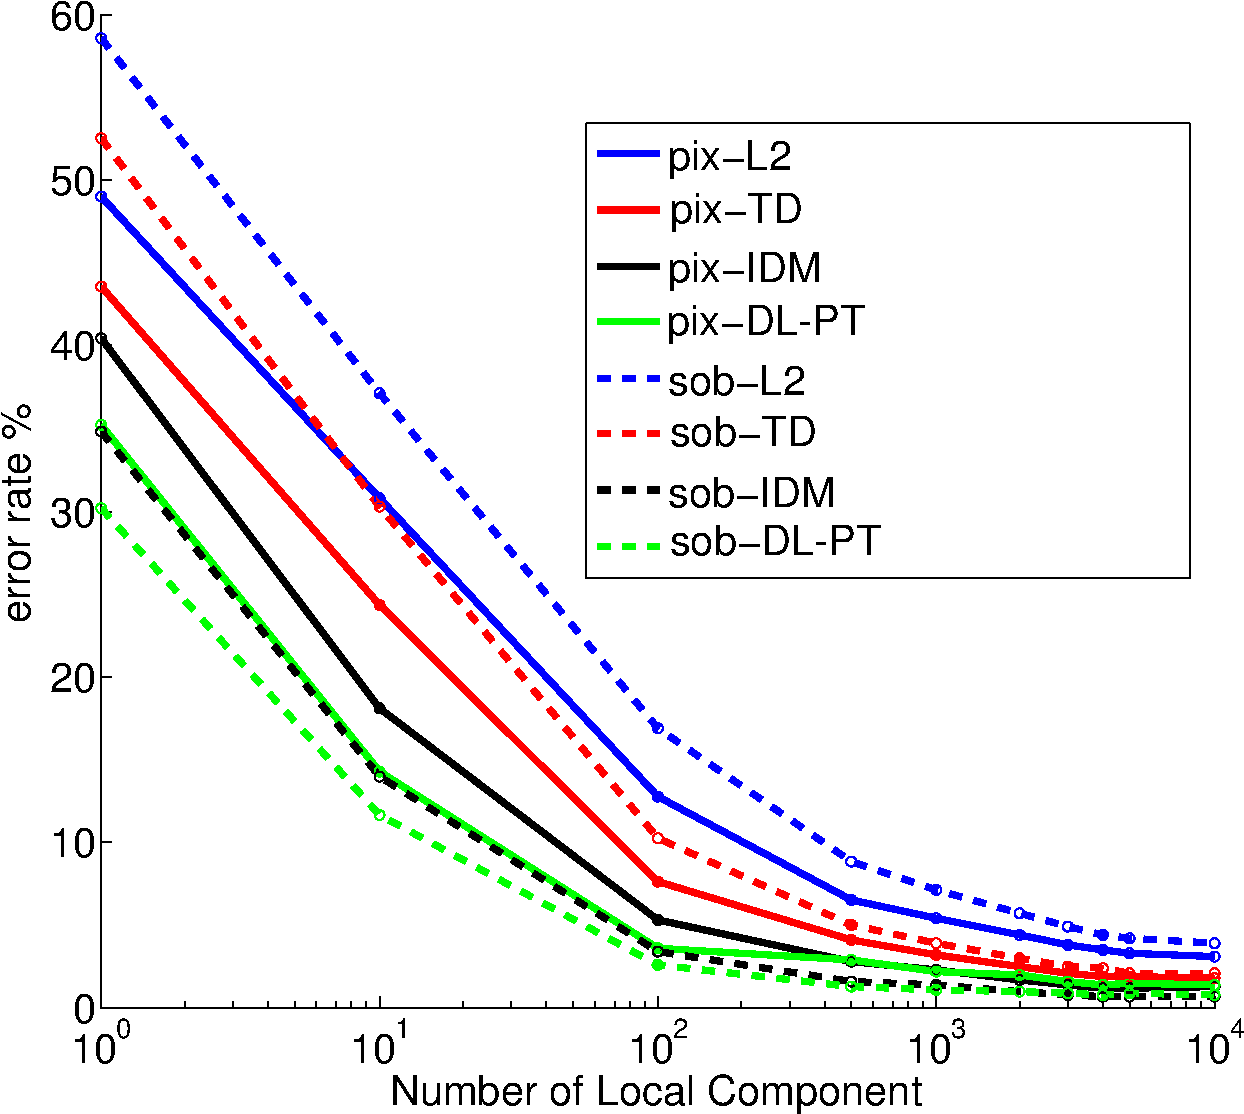
\includegraphics[height=0.7\columnwidth]{figs/f1_err1.pdf}
    \caption{Filled Line: Recognition error on MNIST dataset with pixel intensity as the feature;
      Dashed Line: Recognition error on MNIST dataset with response from Sobel filter as the feature.}   
    \label{fig:char_reg}
\end{figure}


\subsection{Image Synthesis}
%
While many image synthesis experiments are designed to demonstrate
super resolution results which are appealing from a human perceptual
standpoint, our primary purpose here is different. Rather, we wish to
show that the basis learned basis, which is shared across the manifold, are meaningful
from a geometric perspective.

\subsubsection{Digit Synthesis.}
%
For example, given the digit manifold learned from MNIST dataset, we are now able
to synthesize new images of digits by applying randomly sampled action
coefficients to randomly sampled prototypes.  In
Figure~\ref{fig:char_syn}, we show the randomly sampled prototype of
each digit in the first column and synthesized new digit images in the
rest of each row. One can see that the synthesized images
generated by integrating along the geodesic of the manifold cannot be
explained by global affine deformation. For example, in the row of digit two, we
can see that there are some basis related to the size of the lower
left circle of the digit.
\begin{figure}[t]
    \centering
    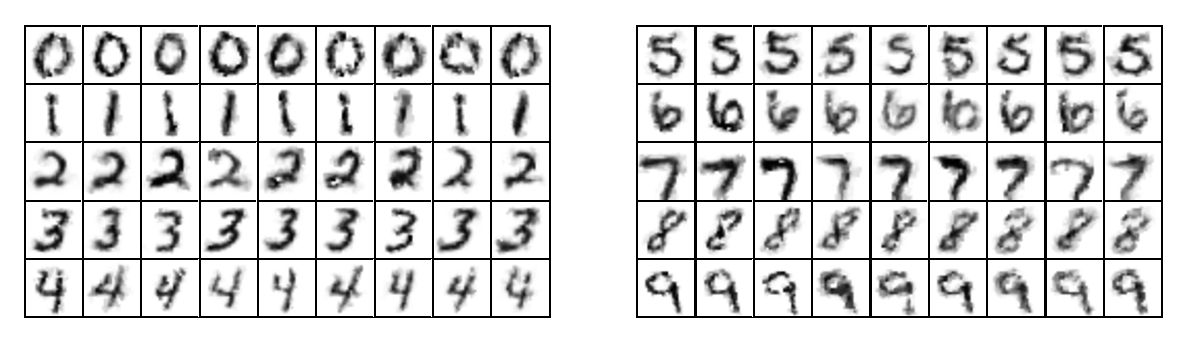
\includegraphics[height=0.28\columnwidth]{figs/digit_table.pdf}
    \caption{Synthesized digits from the learned digit deformation manifold. 
The first digit in the row is the prototype; 
the rest are locally deformed from the prototype with a random coefficients of the learned basis}
    \label{fig:char_syn}
\end{figure}

\subsubsection{Face Reconstruction.}
%
In addition, we learn a face manifold using
the face dataset of Brendan Frey, containing around
2,000 20 by 28 gray scale images of Frey's face in different
expressions and angles of view.  For this experiment, we first learn
the commonly shared basis to contruct the manifold from 1,000 sampled
images.  Then, for a separate set of randomly sampled 500 testing images,
we try to see how close they can be projected onto the manifold.  We
tested three different algorithms for reconstruction: nearest training
image in Euclidean metric, closest projection onto tagent spaces and
closest projection onto our connected deformation manifold with shared
basis.  Again, we test our results with a varying number of
prototypes. Shown in Figure~\ref{fig:face_syn}, we can see that the in
terms of both Euclidean distance and PSNR ratio, the reconstruction
from the manifold with a learned shared basis is consistently better than
those learned independently from training examples. Note that the images
are by themselves small and most reconstruction errors are not human
detectable. Consequently, we do not show the reconstructed faces.

\begin{figure}
    \centering
    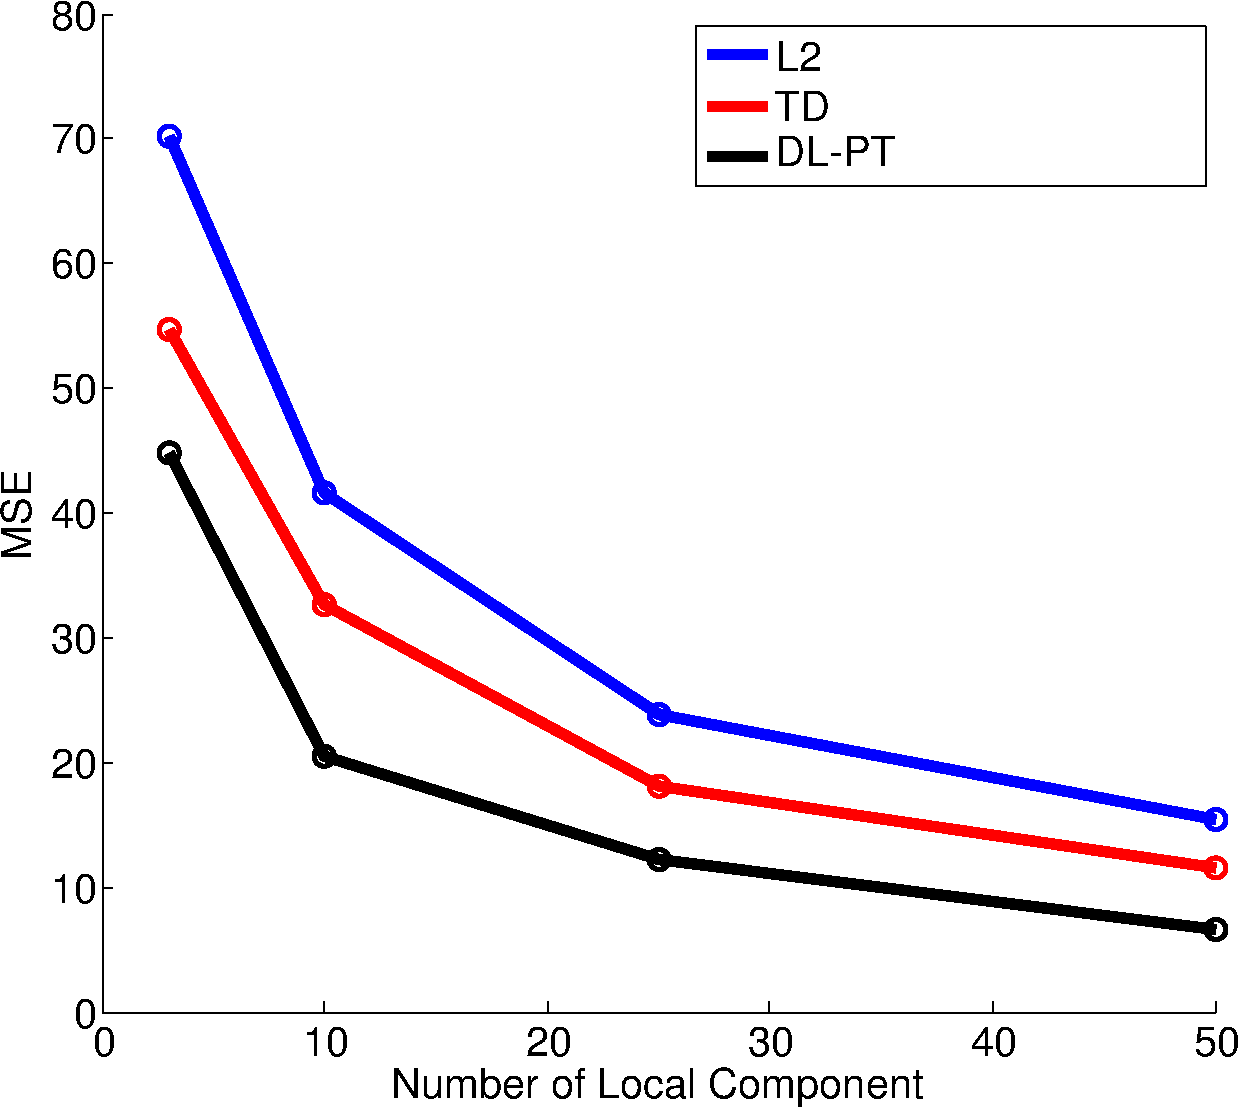
\includegraphics[height=0.4\columnwidth]{figs/f3_mse.pdf}
    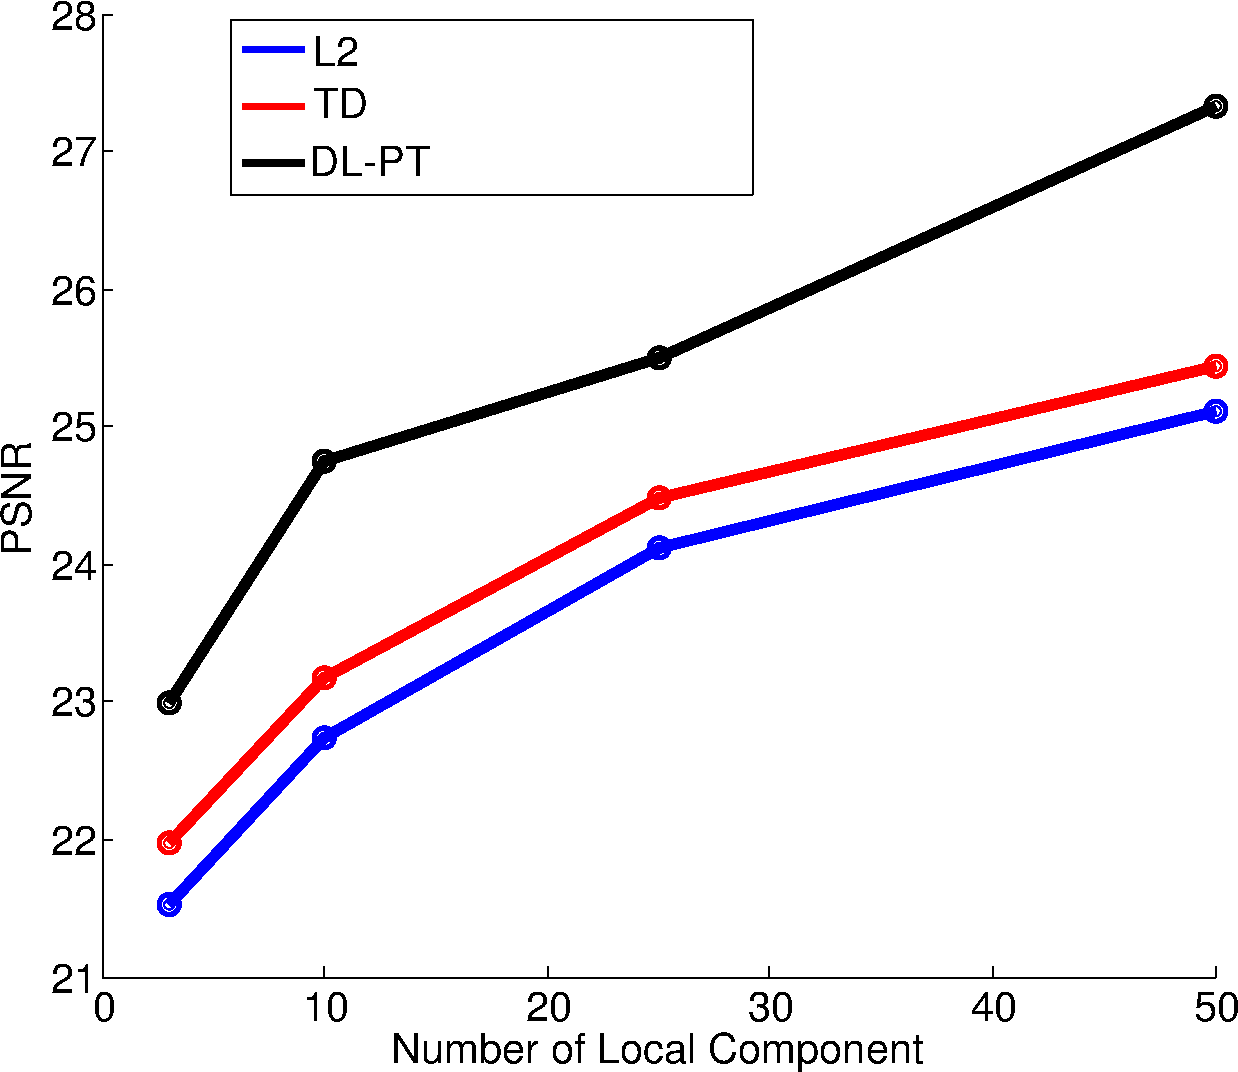
\includegraphics[height=0.4\columnwidth]{figs/f3_psnr.pdf}
    \caption{Comparison of reconstruction performance on face synthesis.}
    \label{fig:face_syn}
\end{figure}

%%% Local Variables:
%%% TeX-master: "main_paper"
%%% End:



\section{Conclusion}
\label{sec:conclusion}
We have presented a new method for manifold learning over images. The
method is distinct from previous approaches in that the model
explicitly incorporates a local Lie algebraic representation of
deformations combined with a consistency relation derived from the
parallel transport property. While previous methods consider local
tangent spaces parameterized by a deformation basis, the methods of
which we are aware utilize a hand crafted basis in contrast to the
presented method which learns the basis. This process was enabled by
exploiting the parallel transport property which imposes geometric
consistency across local tangent spaces and effectively leverages the
full training set (rather than local clusters) for learning properties
of the deformation manifold. An efficient coordinate descent algorithm
was presented along with a suggested initialization
procedure. Empirical results demonstrating the utility of the
methodology were presnted for hand written character recognition and
synthesis as well as human face reconstruction.
%
%%% Local Variables:
%%% TeX-master: "main_paper"
%%% End:


\bibliographystyle{splncs}
\bibliography{deform}

\end{document}
